\chapter{Problem description}
\label{chap:problem}
% 1. As discussed in the introduction in order to facilitate the digital economy in the future an open, distributed reputation system is required. The reputation system will enable trustful relationships between strangers and will need to be at the core of the internet itself.  
% In the introduction we have made a case for our audacious ambition to design and create a layer 
% of reputation on top of the core infrastructure of the internet that enables application agnostic 
% trustful relationships between relative strangers. This requires a distributed, scalable reputation
% system. 

Our audacious ambition is to create a global trust system. Such a trust system as a public, free and 
non-profit utility is a key element to enable next-generation online applications. In the 
previous chapter we have introduced trust research and influential role trust plays in human 
society. The complexities of the design of such a system reach far beyond the scope of a single 
master thesis. In this chapter a specific problem will be defined that we identified as a crucial
challenge to solve in order to achieve the long-term goal.

\section{Model of trust and reputation}
Trust comes natural to people. Our intuition tells us from experience or some evidence who is 
trustworthy and who is not. This is not a failsafe process but it is the best we can do. If we try
to reason about this vague concept of trust or try to implement trust into an automated agent we
cannot use that intuition. Instead a model is needed which describes in explicit terms the 
concepts, and the relationships between them. This helps us to afterwards determine the components 
that are needed to create a fully capable trust system.

"A Computational Model of Trust and Reputation" by Lik Mui~\cite{mui2002computational} is an
important early work which provides a complete computational basis for those vague concepts. Mui
defines the concepts of trust and reputation in the context of an embedded social network. The 
network consists of a set of uniquely identifiable agents that are able to interact with each other. 
Mui's model further describes the interactions as encounters in which each agent performs either a 
positive action "cooperate" or a negative action "defect". This matches the actions from the 
Prisoner's dilemma game that we introduced to the reader in Section \ref{sec:prisoner}. The incentive
for an agent to cooperate in an encounters is the hope that the same agent in future encounters will
return the favor and also cooperate. This is the concept of direct reciprocity which was
mentioned in Section \ref{sec:evolution}. Throughout their lifetime agents build a
history of encounters. The reputation of an agent is determined by that history. A high amount of 
positive reciprocative behavior in the past results in a positive reputation. Mui defines reputation as ``
perception that an agent creates through past actions about its intentions and norms''. A good 
reputation leads to trust from other agents. Mui's definition of trust as ``a subjective expectation
an agent has about another's future behavior based on the history of their encounters'' reflects
this. Mui specifically bases the trust of one agent in another on the personal history between the
two. We will later discuss the case when the complete history of an agent is taken into account. The
more trust an agent has in another, the higher the probability for reciprocation in the following
encounter. This leads to another encounter of reciprocation, effectively increasing the agents 
reputations. This circular relationship is represented in Figure \ref{fig:mui}. 


\begin{figure}[h!]
    \centering
    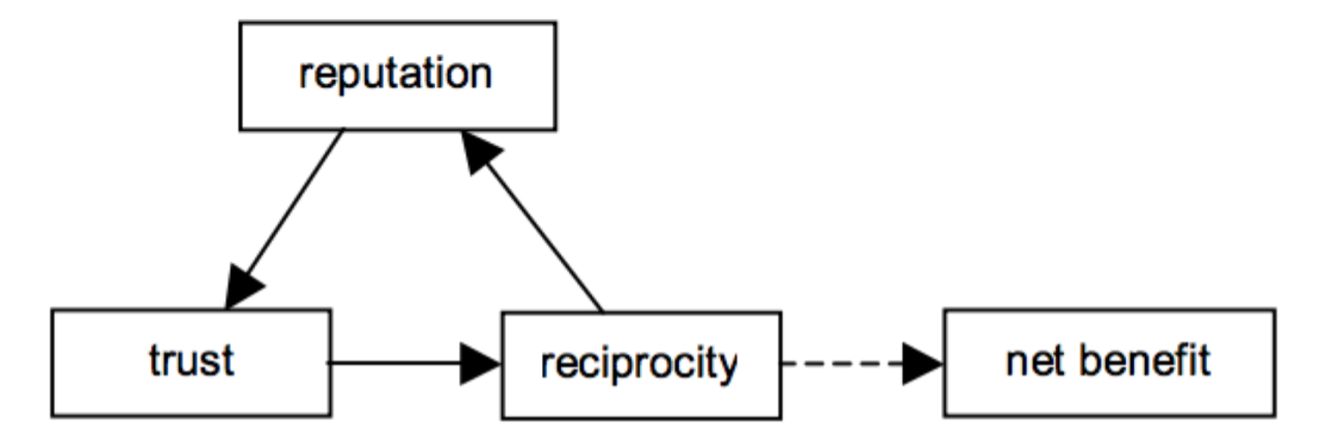
\includegraphics[width=\textwidth]{images/mui_figure}
    \caption{Circular relation between trust, reputation and reciprocity. Source: Mui, 2002~\cite{mui2002computational}}
    \label{fig:mui}
\end{figure}


In Mui's model, trust and reputation can be calculated. For example, an estimator for the reputation
of an agent can be the number of encounters in which the agent reciprocated over the total number of 
encounters. Trust, is the probability that an agent will reciprocate in the next encounter given 
the agent's history. This allows agents who are not guided by human intuition to make automated 
trustful decision. We will use the concepts and implications from this model in the next section 
to define the components which are necessary for the creation of a trust system.

\section{System architecture}
{\color{red} Needs some work to fit better with the previous section}
As of today, no single algorithm or architecture can provide a solution that conforms with all these 
requirements. Only by combining multiple components and iterating their design can we approach a 
reputation layer that is able to conform with the requirements. This layer needs to combine these
components:

\paragraph{Identity.} At the lowest level there is the identity layer that ensures an entity is 
identifiable for other entities in the network. The most basic version of this is a simple public-
private key pair for signing and encrypting data. But creating a new key pair is cheap, therefore 
this is not enough and in a later iteration of this identity system digital entities will need to be 
bound to real-world, verified entites like government-issued passports or biometric identifiers.

\paragraph{Communication.} The internet creates a global communication network with high connectivity
across the world but it is currently not in a state that direct communication between devices is 
straight-forward. The large increase in connected devices expended the address space of IPv4 and IPv6
transition has been slow, thus network address translation creates subnetworks with local address 
spaces. Connection from such a subspace to a server with a public adress is still simple like it is
the case with most client-server applications on the internet, but direct communication when both 
devices are behind NATs is still not standardized. Also new routing solutions are required to ensure
communication based on the actual identity layer mentioned before instead of the IPv4 and DNS identity
layer.

\paragraph{Record and distribution mechanism} Reputation is based on feedback on interactions. 
This feedback needs to be recorded and distributed, such that other entities in the
network have a chance to respond to the history of feedback of their peers. Without a central entity
which is aware of all transactions, each node will record some transactions. It is a challenge to 
create a global record which is correct, tamper-proof and well distributed across the network.

\paragraph{Interpretation of records} Based on the recorded feedback each agent can interpret them
to form an opinion about other nodes. For a reputation system the records are seen as positive or
negative behavior and each agent can output a ranking of reputations for all peers this agent knows
of. Those rankings are calculated based on a reputation function. In the past our research group has
analyzed different reputation functions like NetFlow~\cite{OTTE2017}, 
MaxFlow~\cite{meulpolder2009bartercast} and PageRank~\cite{page1999pagerank}.

\paragraph{Application layer} We imagine that the reputation system we are developing can be used 
for any type of application that requires two entities to trust each other. This reputation layer 
will be accessible for anyone however no application will be able to delete data or lock data into
their proprietary platform. 

%     \item identity layer: digital identities are related to real-world entities and can either be real-people or entities like institutions or companies. The most simple first solution is just to identify entities by their public-private key pair.
%     * encounter record and distribution layer: encounters between digital identities needs to be recorded and distributed. Encounters are the basis for the reputation of entities, but reputation is only useful if it is gossiped such that other people can make decisions on the knowledge they have.
%     * interpretation layer: based on the known history of encounters, a reputation can be given to the known entities and decisions can be based on this. This layer contains the reputation function: NetFlow, MaxFlow, PageRank etc.

Each layer adds another level of protection: if identities are expensive and hard to create, fake 
identities will be less easy to create, protecting the system against spamming. Creating an immutable
record and distributing that information to everyone makes knowledge tamper-proof, unchangeable and 
forever, making all information reliable. On the interpretation layer additional securities can be 
enabled: we envision a concept of locality to secure against distributed attacks with global 
collaborations of malicious nodes - if we only trust agents with a certain level of latency 
attackers can only choose from nodes in the vicinity and supply of those nodes is limited. 

\section{Value of reputation}
The concept of trust is however vague. In the analog world, trust is more of a feeling than a 
rational calculation, yet computing systems are deterministic, precise and rational. The vagueness 
partly stems from the subjective interpretation of actions which in the digital system is the 
reputation function used, but also from the difference in what each person knows about another one,
or in digitally speaking subsets of information that each one agent has. 
Yet, from a practical point of view it would be desirable if people could agree on the reputation 
and trustworthiness of agents, because it makes actions predictable and gives reputation its value. 

To see this we should go back to the discussion of indirect reciprocity, which is one of the five
forms of fostering cooperation which were introduced in chapter~\ref{chap:introduction}. People act
pro-socially at a personal cost in order to build an altruistic reputation which is rewarded with 
third-parties acting pro-socially towards them. Reputation is valuable because people with higher 
reputation can expect more cooperation in future interactions. This indirect reciprocity mechanism 
works as long as agents agree on what is good and what is bad reputation. Once there is ambiguity 
about the reputation of agents this value decreases as even people with a bad reputation could be 
seen as good people by others due to that ambiguity. Also only if reputation has actual value to 
agents, we can ensure pro-social behavior in the network. Therefore we need agreement on the 
reputation of agents. 

Agreement on the interpretation layer can be achieved by defining a function for all agents to use
which calculates a quantitative reputation from the history of feedback. Usually this history is 
public, visible to everyone, however this is difficult to achieve in a distributed system. Here the
second problem comes into play. The information a network node acts upon 
is a different subset of complete information on the network for each agent; each agent is 
in a different state. This situation is undesirable but inherent to systems with the requirements 
stated in the previous section. Thus, a first step towards agreeing on the reputation of agents is 
if agents agree on which data should be used as an input to the reputation function. In 
other words we have to make sure that agents disseminate their knowledge and obtain knowledge from 
other agents such that information is well distributed and available.

However, in most contexts sharing and obtaining information comes at a cost which is not negligible.
Thus agents may be reluctant to spend resources without any direct reward. There is an obvious 
network effect to agents knowing more about their peers but agents can also gain reputation by 
cooperating with agents with low reputation. Thus there is no incentive to obtain a better view of
the network.

\section{Research question}
The design of a global trust system bears many challenges. A lot of research has gone into the
development of algorithms for calculating trust and models for the behavior of agents in the presence
of trusted and distrusted agents. However, we found that the basis for trust is reputation, which in 
turn is based on the records of encounters. Yet, recording, distributing and securing
the information about encounters in distributed systems is an underexplored topic and has only 
little literature published in the scientific community.

Consequently, the question that we are trying to answer is therefore:
\begin{center}
    \textit{How to record, disseminate and protect the records of interactions in a global trust system?}
\end{center}

\section{Requirements of reputation systems}
Reputation systems appear in many forms but we are concerned with their digital form as only
digital networks can reach global scale with fast information distribution. Reputation systems have
previously been formally defined to include at least three components \cite{resnick2000}:

\begin{itemize}
    \item Long-lived identities
    \item Recording and distribution of feedback about interactions
    \item Use of feedback to guide interactions
\end{itemize}

We need entities to be identifiable and in existence for a long time to ensure that future interactions
between known entities are likely. If changing of identities is easy, a bad reputation is easily 
discarded and exchanged for a clean slate. We need to capture and distribute feedback of interactions
such that entities are aware of the history and reputation of other entities on the system. Finally,
users should actually make use of the feedback on not just ignore it.

\section{Requirements of global trust system}
Next to the requirements of reputation systems we also have requirements for specific use case of a
global reputation system without centralized institutions.

% 2. The reputation system we define needs to have some properties:

\begin{itemize}
    \item distributed: no entity should be owner of the reputation of all people, no single point of
    failure should exist
    \item scalable: future applications similar to those that exist today with centralized reputation
    systems should be able to handle billions of users.
    \item robust against strategic manipulation: once reputation increases in worth users of the 
    system will try to exploit the system by attacking it, alone or by colluding and the
    architecture needs to be robust against such attacks
\end{itemize}
  
This introduces additional challenges: enforcing long-lived identities is even harder without the 
assumption of a trusted central entity that can check the validity of new entities. Also creating
a central distributed record with synchronization at scale is a topic of ongoing research and 
generally seen as an unsolved problem. Finally, reputation system in general and distributed systems
specifically are intrinsically weak in protection against malicious behavior, although they are 
robust in terms of complete failures as no single point of failure exists.

\section{Related work}
{\color{red}
\begin{itemize}
    \item First and second generation crypto currencies
    \item Reputation systems
    \item Dissemination mechanisms
    \item Conclusion nothing does it all
\end{itemize}}

% In the previous two chapters we have shown that a need exists for a decentralized accounting system 
% in order to create a global infrastructure for secure, anonymous digital transactions that does not 
% require control through a trusted third party. This need has been identified before and work has 
% been performed both in the scientific community as well as the industry. In this chapter we will 
% summarize those efforts, describe the short-comings of those approaches and define a basis for the 
% work performed in this work.

% \subsection{Dissemination mechanisms}
% Achieving the desired dissemination of transaction records is not a new problem in distributed 
% system as it is similar to synching the two stateful disconnected systems, for example a database.
% Dissemination mechanisms have been researched for many decades. \cite{hedetniemi1988survey} is an 
% early summary of the most important techniques in on dissemination Hedetniemi et al. describe 
% gossiping, broadcasting and shortly mention receiving and polling. We shall briefly introduce the 
% concepts here.

% \paragraph{Gossiping} Gossiping is the a mechanism in which pairwise exchange of information takes 
% place. Imagine a set of agents in which each agent has knowledge of a unique set of encounters that
% all other agents are not aware of. The goal is to reach a state in which all agent have the
% information on all encounters. During gossipping, an agent chooses a set of partners and with each 
% partner the agent exchanges all information. This is done by each agent and after a certain number
% of interactions the dissemination is complete. Different variants exist for gossiping, for example
% only allowing one-way communication, allowing multi-party exchanges and restricting the number of 
% exchanges per agent. 

% \paragraph{Broadcasting} Broadcasting is a process in which information originates from one 
% agent in the network, who needs to transmit the information to all other agents in the system. Again
% information transmission happens in pairs of two agents, and communication only happens between 
% adjacent nodes in the network. In contrast to gossiping where new information originates at all 
% nodes, in broadcasting all nodes communicate one piece of information.

% \paragraph{Receiving} In receiving all agents send some unique information to a specific agent, called
% the receiver. 

% \paragraph{Polling} Polling a information accumulation process in which a single originating agent sends requests for
% information to all other agents who then respond with an information carrying message. 

% The survey shows that dissemination of information in itself is a well understood topic and many 
% implementation of such protocols are widely available. However some problems exist when taking into
% account the possibility of strategic manipulation. Those will be discussed in the next section.


% \subsection{Decentralized accounting systems}
% The general concept of accounting is quite old as it is simply a recording of transactions between
% two or more parties. Before the digital age those recordings were simply written text on paper, 
% nowadays those recordings are stored in databases. We are concerned with another type, namely 
% decentralized accounting systems. We identified three types of applications for decentralized 
% accounting systems: cryptocurrencies, distributed work systems and reputation systems. 

% In the years 2007 and 2008 the global financial crisis shattered the global economy, lead to many
% people loosing house and job and diminished the trust clients had in banks to keep their money safe.
% Politics discussed the problem and proposed to regulate the banks more but with little impact. 
% However something else promised to change the banking world: the first white-paper for a 
% decentralized digital currency without any need for a trusted third party, Bitcoin, was announced. 

% \paragraph{Bitcoin.}
% Before the announcement of Bitcoin it was assumed that in order to verify the correctness of 
% transactions between parties and prevent cheating with digital money a bank or credit card company
% was needed. Bitcoin proved them wrong by creating a hash-based chain of transaction blocks, a global 
% ledger, that is shared among all users of the network. The acceptance of transactions is managed by 
% a process called ``mining'' which ensures that only the majority of CPU power can publish new 
% block. A blocks contains a fixed number of transactions and the Bitcoin network makes sure that a
% block is created once every 10 minutes. All mining node will execute the proof-of-work mechanism: 
% in order to publish a block a value needs to be found that, when hashed with a certain hashing 
% function like SHA-256, starts with a certain number of zeros. Depending on how many CPUs are active
% on the network the problem can be increased in difficulty by requiring more zeros at the beginning 
% of the hashed value. Once a new block is published other nodes will validate the transactions and 
% if they agree, will show their acceptance by working on creating the next block. This system ensures
% that as long as a majority of CPU power is owned by honest nodes, they will outpace the rest of the
% network in solving the hashing puzzle and creating valid blocks. Nodes will accept the longest chain
% and the transactions will be valid.

% The Bitcoin approach solved many problems assuming that an honest majority exists: first and 
% foremost the double-spending of funds is prevented because the Bitcoin blockchain creates one global
% order of valid transactions. Also the Sybil-attack is prevented by pairing the voting power to the
% available CPU power, which means Sybils can only run on real hardware, removing the advantage of
% fake identities. But these measures of attack prevention come at a price of efficiency. The surging 
% price of Bitcoins especially in the year 2017 led to a surge in transactions, transaction fees and
% energy usage. The increasing price of Bitcoins makes mining them more profitable which means more 
% nodes are joining the mining operation. Therefore the difficulty for the proof-of-work problem is 
% increased, such that it takes more computing power to find a correct value. This again increases the
% amount energy consumed in the whole network. At the same time the number of transactions processed
% is a constant of the Bitcoin currency, approximately 7 transactions per second. At the time of 
% writing the energy conusmption is at least 2.55 GW which makes it comparable to contries such as 
% Ireland. Summarized Bitcoin was a large step towards decentralized accounting but unsolved 
% scalability issues still prevent it from being actually useful as an infrastructure such as the one 
% we envision.

% \paragraph{Alternative coins and improvement measures.}
% Bitcoin served as a first proof-of-concept for trustless digital currencies or for our purposes, a
% ``secure'' decentralized accounting system, but the shortcomings were also obvious. Once the 
% populartiy increased, other enthousiasts, startups and incumbent companies started to create their 
% own spin-off digital currency. Each of these so-called ``alternative coins'' used blockchains as 
% a core technology to store transactions but tried to solve the scalability issues using different 
% approaches. The discussion of all alternative coins goes beyond the scope of this chapter, therefore
% we will quickly introduce some of the main differences between the largest systems. 

% The block time is one parameter to tweak in order to increase transaction throughput. Ethereum, the
% second largest cryptocurrencies currently uses a block time of 15 seconds with a proof-of-work 
% consensus. Also block size is a factor in the throughput rate, but increasing block time and size 
% only creates a constant factor to the rate of transactions.

% Ethereum is currently testing a proof-of-stake mechanism which should replace the energy intesive 
% proof-of-work. In short this mechanism will require ``minders'' to put some amount of currency into
% a wallet in order to participate in the process. If a miner does not perform the validation of 
% transactions correctly that ``stake'' will be lost for the miner. This will solve the energy 
% consumption problem but it will not solve the overall scalability issue of the system. 

% Another feature in development in multiple currencies is the ``Lightning network''. The lightning 
% network will allow two parties that expect to conduct multiple transactions with each other to 
% create a ``channel''. Both parties store some funds in the channel and can then interact freely 
% through this channel without needing to interact with the master network of the currency. Only the
% opening and netbalance at closing time will be writting to the chain while all other interactions 
% are only recorded locally. This should increase the possible throughput significantly but due to the
% early stages of development the actual implications of large-scale use are not proven at the time of
% writing. But considering that Bitcoin has a transaction limit of 200000 transactions a day, it would 
% still take 5000 days or 13.7 years to open one channel each for a billion people.

% The IOTA project ...

% Sharding ...

% Conclusion is no other system exists that fulfills the requirements


% \subsection{Distirubted work systems}
% In the field of distributed computing many applications include some mechanism in which a node is
% performing work for other nodes or the network in general. Seuken et al. call these distributed 
% work systems. Some examples of distributed work systems are peer-to-peer file-sharing network,
% packet forwarding in mobile ad-hoc networks and volunteer scientific distributed computing. As our 
% research group is mostly concerned with file-sharing networks and the concepts are similar in 
% general we will stick to that example to discuss the latest developments.

% Many different file-sharing networks have been built in the past, the most prominent being Napster,
% Gnutella and BitTorrent. In contrast to centralized file-sharing, in peer-to-peer systems there is 
% no server that contains all data, but instead users share data directly, one peer downloading and 
% one peer uploading. With no infrastructure needed, no costs and no single point of failure such a
% systems seems optimal. Talking in terms of distributed work systems, the act of uploading is 
% equivalent of performing work while the act of downloading consumes work. There is, however, a 
% social dilemma here: uploading to another node does not lead to an immediate reward for the
% uploading node, therefore, if we assume that bandwidth is a precious resource it is cheaper to not 
% upload, yet if all agents on the network realize this, no agent will upload and thus no agent is 
% able to download. The agents that do not upload any data are known as free-riders and free-rider 
% protection in peer-to-peer file-sharing networks is a subject of ongoing research.

% Accounting systems pose a possible solution to the free-riding problem. Let's first imagine a 
% centralized accounting systems keeping track of all uploading and downloading behavior, uploading 
% data increases the balance of agents, downloading decreases the balance. Now, the accounting system
% can enforce that agents keep their balance around 0, so they upload approximately as much as they
% download. Therefore, an accounting system can solve the free-riding problem, however as mentioned 
% multiple times, a decentralized accounting system is hard to implement. Accounting mechanisms have
% first been related with this subject in the DropEdge paper, however a lot of work has been done on
% the very related subject of reputation systems, which will be discussed in the next section. Seuken
% et al. define an incentive-compatible accounting mechanism which removes any advantage for users 
% that misreport their own contributions in the network. They present their DropEdge algorithm and 
% show that it's possible to increase the efficiency of BitTorrent clients using accounting. A 
% negative result of their work is that an accounting mechanism cannot prevent sybil attacks. Some
% short-comings of the approach is strategic manipulations of data and dissemination of data. 

% \subsection{Reputation systems}
% One of the reasons that decentralized accounting systems are hard to create is that agents in
% peer-to-peer applications do not have a complete view of the network and thus also not all 
% information of the network, at least not without a global consensus mechanism. In the file-sharing
% example from the previous section agents decide to upload to other agents based on some partial 
% knowledge of the network and contributions of agents. It can be argued that an accounting mechanism
% cannot be correct if it acts on partial information and instead the particular balance of an agent 
% as seen by another agent is rather a reputation. The goal is then to create trust between users in 
% order to facilitate cooperation. Such a system will be called a reputation system. 

% Whether reputation systems can be called an application of accounting systems can be argued about. 
% In general accounting systems track transactions between accounts, the full history of transactions
% determines the state of the network. According the framework of Mui et al. trust is the expectation
% of reciprocation for an agent given that agent's history of behavior. So a reputation system can act 
% on the data of an accounting system and add additional conclusions. The previous example of agents
% uploading and downloading helps to understand this. An accounting system keeps track of the 
% transactions and calculates the balance of an agent, for example +10MB, for an agent that has 
% uploaded 10MB more than downloaded. Also it is possible to account the total uploaded and downloaded
% data, for example 1010MB and 1000MB respectively. A simple accounting system stops at this point, 
% the system behaves correctly when no error has been done in calculating the balances and the data is
% correct. A reputation system adds another layer of interpretation to this data. The simplest 
% reputation function only checks whether the balance is positive or not, or if the choice is between
% multiple agents, whose balance is the most positive. Another reputation function might weight agents
% with a 0 balance but 10GB of uploaded (and downloaded) data more trustworthy than an agent with 10MB
% positive balance but only 100MB uploaded data. Thus we can see a reputation system as a layer on top
% of an accounting system.

% Describe some reputation systems ...
\section{Agent behavior through incentive}

\section{Scope}